\documentclass{article}
\usepackage[left=2cm,right=2cm,top=2cm,bottom=2cm]{geometry}
\usepackage[utf8]{inputenc}
\usepackage[german]{babel}
\usepackage{amsmath}
\usepackage{dsfont}
\usepackage[export]{adjustbox}
\usepackage{amsthm}
\usepackage{color}
\usepackage{amsfonts}
\usepackage{amssymb}
\usepackage{wasysym}
\usepackage{makeidx}
\usepackage{graphicx}
\usepackage[colorlinks=true,urlcolor=blue,linkcolor=blue]{hyperref}
\usepackage{ziffer}
\usepackage{minted}
\usepackage{xcolor}
\usepackage{framed}
\usepackage{mdframed}
\usepackage{subfiles}
\usemintedstyle{emacs}

\definecolor{purp}{HTML}{9A72AC}
\definecolor{re}{HTML}{FC6255}
\definecolor{gre}{HTML}{83C167}
\definecolor{blu}{HTML}{58C4DD}
\definecolor{shadecolor}{rgb}{0.85,0.85,0.85}
\definecolor{bg}{rgb}{0.95,0.95,0.95}
\setlength{\parindent}{0em} 

\BeforeBeginEnvironment{minted}{\begin{mdframed}[linewidth =2 ,backgroundcolor=bg , linecolor=black, linewidth=0.5]}
\AfterEndEnvironment{minted}{\end{mdframed}}

\newtheorem{defi}{Definition}
\BeforeBeginEnvironment{defi}{\begin{mdframed}[linewidth =2 ,backgroundcolor=bg , linecolor=black, linewidth=0.5]}
\AfterEndEnvironment{defi}{\end{mdframed}}

\newcommand{\bsp}{\textbf{Beispiel}:}
%\newcommand{\task}{\textbf{Aufgabe}:}

\newcommand{\bol}[1]{\textbf{#1}}
\newcommand{\q}[1]{\glqq #1\grqq}
\newcommand{\DODO}[1]{\textbf{\textcolor{red}{DODO:}} #1 \\ \begin{center}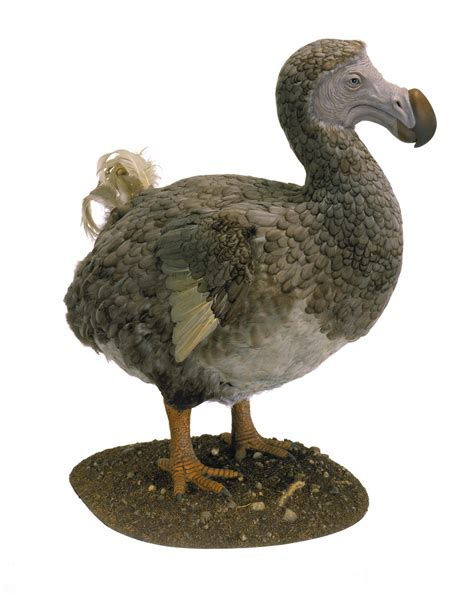
\includegraphics[scale=0.2]{../../media/dodo.jpg} \end{center}}

\newenvironment{task}[1]{
    \begin{shaded*}
    \textbf{Aufgabe #1}:
}{
    \end{shaded*}
}

\begin{document}

\subsection{Rahmenbedingungen}

Und jetzt zur eigentlichen Aufgabe, in einem Satz:

\begin{task}{- das Projekt}
Entwickeln Sie in Dreierteams ausgehend von einer eigenen Problemstellung mit Hilfe agiler Methoden ein Programm, das sich am Architekturmuster MVC orientiert.
\end{task}

\textbf{Wichtige Punkte vorweg}:
\begin{itemize}
    \item Voraussichtliches Startdatum: 2.5.23
    \item Voraussichtliches Enddatum: 27.6.23
    \item ersetzt kleinen praktischen Leistungsnachweis
    \item Dreiergruppen (keine Ausnahmen)
    \item Abschlusspräsentation/Vorführung des Programs bzw. des aktuellen Standes
    \item Jeder in der Gruppe muss beitragen $\Rightarrow$ Jeder ist verantwortlich für einen der drei Bereiche Model, View oder Controller. Das bedeutet \textbf{nicht}, dass zwangsläufig alles in diesem Bereich von derselben Person programmiert werden muss. \\
    \textbf{Aber}: Nachfragen im konkreten Bereich müssen vom Verantwortlichen in der Abschlusspräsentation beantwortet werden.
    \item Der Code des Projekts muss \textbf{ausführlich kommentiert} werden. Im Zuge der Bewertung ist diese Vorgabe notwendig, auch wenn sie dem agilen Manifest widerspricht. Desweiteren müssen grob die von den einzelnen Teammitgliedern bearbeitenden Aufgaben klar werden (Details bei \hyperref[sec:hwUserStories]{\textbf{User Stories}}, \hyperref[sec:git]{\textbf{Git}} oder Punkt 4 des Fahrplans). Als Ausgleich muss \textbf{keine weitere} Dokumentation der \textbf{Arbeitsweise} in der Gruppe (z.B. als Portfolio) erstellt werden.
    \item \textbf{Für die Experten}: Die Programmiersprache muss nicht zwingend Java sein, es muss aber in der Gruppe Konsens bezüglich der Sprache herrschen. Bei geplanter Abweichung von Java zunächst auch Rücksprache mit der Lehrkraft notwendig. Der Fokus liegt auf \textbf{Objektorientierung}.
    \item Es sollen \textbf{mindestens} für dei wichtigsten Funktionen, in jedem Fall aber für die gesamte Anwendung Tests vorhanden sein.
    \item Die Zeit während des Unterrichts reicht (in den meisten Fällen) nicht aus für ein sehr gutes Ergebnis!
\end{itemize}

\textbf{Fahrplan}

\begin{enumerate}
    \item \textbf{Ideensammlung}: Das Team überlegt sich gemeinsam welche Art von Program erstellt werden soll und \textbf{einigt sich} auf ein grobes Ziel.
    \item \textbf{Erste Erstellung von User Stories}: Zuerst sehr grob: \q{Was soll das Programm können?}. Für Details siehe entsprechendes  Unterkapitel.
    \item \textbf{Besprechung und Entwurf}: Besprechung mit Lehrkraft $\Rightarrow$ Absegnung des Projekts, parallel: Beginn der groben Planung, z.B.: wird eine Datenbank benötigt, welches Framework für die GUI, etc., grobes Klassendiagramm der benötigten Komponenten (siehe auch \hyperref[sec:hwModel]{\textbf{Model}}, \hyperref[sec:hwView]{\textbf{View}}, \hyperref[sec:hwController]{\textbf{Controller}})
    \item \textbf{Arbeitsaufteilung - Organisation Sprint}: Konkretisierung der User Stories, gegebenenfalls Aufdröselung in die drei Teilgebiete, Erstellung von Aufgaben (\textbf{Issues} oder \textbf{Tasks}), die im nächsten Sprint abgearbeitet werden sollen, sowie deren Priorisierung. \\
    Die Aufgaben können entweder handschriftlich fixiert werden oder entsprechende Tools verwendet werden, z.B. \textbf{\href{https://trello.com/}{Trello}},\textbf{\href{https://www.notion.so/de-de}{Notions}} direkt \hyperref[sec:git]{\textbf{Github}}, oder andere tools.
    \item \textbf{Sprint}: Eigentliche Implementierungsarbeit, dabei immer wieder Austausch am Beginn der Unterrichtszeit. (\textbf{Daily Scrum} - \textbf{Standup-Meeting})
    \item \textbf{Sprint-Retrospektive und Neudefinition}: Etwa alle 1,5 Wochen: Rückblick - was ist geschafft? Neue Aufgaben verteilen. 
    \item \textbf{Arbeit!} Wiederholung von 4 bis 6. 
    \item \textbf{Abschlusspräsentation}: Vorstellen des eigenen Programms, Rückfragen zum Code beantworten. 
\end{enumerate}


\subsection{Bewertungskriterien}
\label{sec:Bewertung}
Bewertet werden folgende Kategorien, jeweils mit Beispielen:

\begin{enumerate}
    \item \textbf{Generelle Umsetzung der Vorgaben (Doppelte Gewichtung)}: wurde tatsächlich MVC als Grundlage verwendet, wurde im Team gearbeitet oder sind es drei Einzelprojekte, wurde der Fahrplan grundlegend umgesetzt, $\dots$
    \item \textbf{Komplexität und Umfang des Programs}: wurde TicTacToe oder doch eher Frogger implementiert, besteht nur eine einfache Funktionalität oder mehrere/eine komplexe, $\dots$
    \item \textbf{Umsetzung und Design}: wurde \q{BruteForce} gecodet oder Konzepte verwendet, wurden die Ziele umgesetzt oder fehlen Aspekte, $\dots$
    \item \textbf{Dokumentation}: selbsterklärend :)
    \item \textbf{Arbeit in der Gruppe und im Team}: wurde über Struktur und Implementierung diskutiert, wurde kollaborativ gearbeitet, $\dots$
    \item \textbf{Abschlusspräsentation}: wurde das Programm vollständig vorgestellt, wurden alle Nachfragen korrekt beantwortet, war der Vortragsstil ansprechend, $\dots$
\end{enumerate}



\subsection{Git und Github}
\label{sec:git}

Um Probleme wie Überspeicherung, Datenverlust, etc. vermeiden, so bietet es sich an ein \textbf{Versionskontrollprogramm} zu verwenden, d.h. ein Programm, dass sich den Stand des Codes zu definierten Zeitpunkten \q{merkt}. Die populärste Variante ist heutzutage \textbf{Git}. \\
Wer nach der Schule professionell programmieren möchte, muss sich zwangsläufig mit Git auseinandersetzen. Im Rahmen dieses Skripts werden nur absolute Grundlagen dargestellt, da alles andere den Rahmen sprengen würde. Ausführliche Tutorials gibt es aber überall im Internet zu finden, ein paar Anlaufstellen:
\begin{itemize}
    \item \href{https://www.w3schools.com/git/git_intro.asp?remote=github}{w3Schools Git Tutorial}: textbasiertes Tutorial
    \item \href{https://git-scm.com/docs/gittutorial}{offizielles Dokumentationstutorial}
    \item \href{https://www.youtube.com/playlist?list=PLNmsVeXQZj7rbmmqb1Lt_RGU4DEhelTrR}{Videoreihe von Morpheus - Deutsch}
    \item Allgemein: Google/ChatGPT/Youtube: ihr wisst wie das geht :)
\end{itemize}


\subsubsection{Git}
Die zentrale Verwaltungseinheit bei Git ist ein sogenanntes \textbf{Repository}. Hier werden alle Daten, die mit dem Projekt zu tun haben abgespeichert. \\
\textit{Hinweis:} Git ist ein eigenes Programm und muss vor Verwendung installiert werden (\textbf{\href{https://git-scm.com/download/win}{Windows-Installer}}.  \\
Git kann rein lokal verwendet werden, d.h man erzeugt z.B. ein neues Repository mit (Hinweis: die Dollarzeichen sind nur ein command prompt symbol und sollen \textbf{nicht} eingegeben werden!): 
\begin{minted}{console}
$ git init
Initialized empty Git repository in /path/to/repository/.git/
\end{minted}
Es wird dadurch ein (versteckter) Ordner erzeugt, in dem git die Versionierung verwaltet (ihr könnt bei Interesse natürlich hineinsehen, ansonsten wird dieser Ordner aber nicht manuell bearbeitet). \\
Nehmen wir an, es wurde eine Datei $test.txt$ im selben Ordner erzeugt, dann müssen wir git mitteilen, dass wir diese Datei \q{tracken} wollen, d.h. ihre Änderungen sollen durch Git überwacht werden: 
\begin{minted}{console}
$ git add test.txt
\end{minted}
Es wird jetzt noch eine weitere Datei \q{test2.txt} erzeugt. Wollen wir Informationen über den aktuellen Status unseres Repositories einholen, können wir $git status$ verwenden:

\begin{minted}{console}
$ git status
On branch master

No commits yet

Changes to be committed:
  (use "git rm --cached <file>..." to unstage)
        new file:   test.txt

Untracked files:
  (use "git add <file>..." to include in what will be committed)
        test2.txt
\end{minted}
Hier werden jetzt einige Informationen angezeigt, der Reihe nach: 
\begin{itemize}
    \item \textbf{No commits yet}: Ein Commit ist in Git eine Aktion, mit der Änderungen am Repository festgehalten bzw. gespeichert werden. Ein Commit enthält also alle Änderungen, die seit dem letzten Commit vorgenommen wurde. Wird etwas \q{commitet}, wird in der Regel eine Nachricht beigefügt, die beschreibt, um was es in diesem Commit ging. 
    \item \textbf{Changes to be committed}: hier stehen alle Dateien, die seit dem letzten Commit geändert wurden \textbf{und} mit git add dem Tracking hinzugefügt wurde. Sie liegen jetzt in der sogenannten \textbf{staging area}:
    \begin{center}
        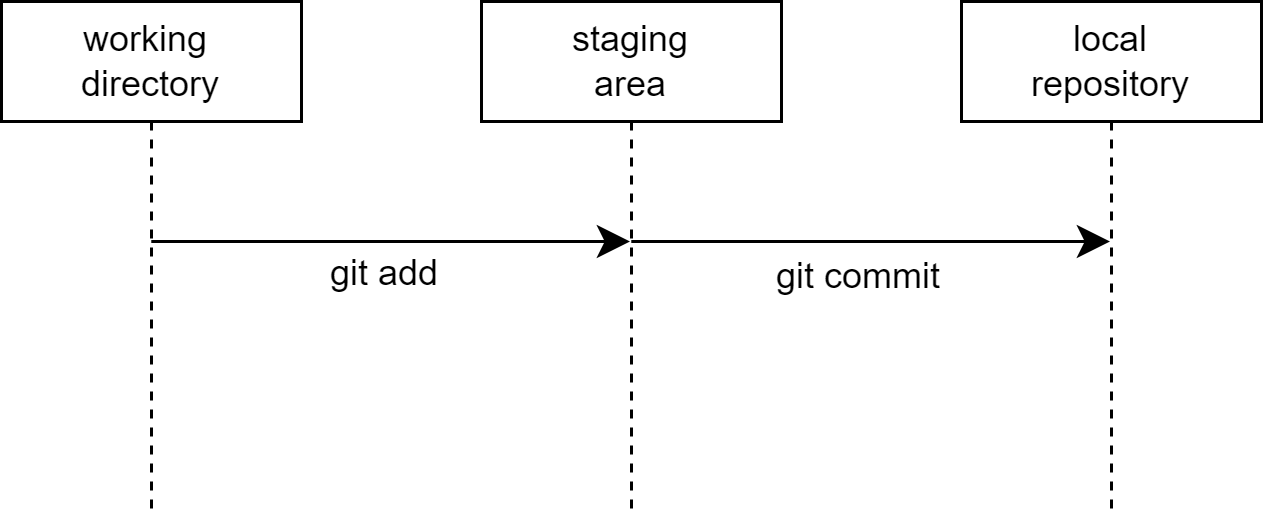
\includegraphics[scale=0.25]{../../media/git_staging.png}
    \end{center}
    In der Staging Area sind alle Dateien zusammengefasst, die getrackt werden, diese können mit einem Commit dem Repository hinzugefügt werden. Das zeigt insbesondere eines: Nur weil eine Datei im selben Ordner liegt, ist sie noch nicht dem Repository hinzugefügt!
    \item \textbf{Untracked Files}: Dies teilt uns auch git status mit, test2.txt liegt zwar in unserem Ordner, wird aber noch nicht getrackt!
    \item \textbf{On branch master}: Dies zeigt uns an, auf welchem \q{\textbf{Zweig}} wir uns gerade befinden, dazu später mehr. 
\end{itemize}

Sind wir zufrieden mit unseren Änderungen, so können wir sie per \textbf{git commit} dem Repository hinzufügen, möchte man noch eine Commit Nachricht hinzufügen verwendet man:
\begin{minted}{console}
$ git commit -m "Das ist unser erster Commit!"
[master (root-commit) 56f4a69] Das ist unser erster Commit!
 1 file changed, 0 insertions(+), 0 deletions(-)
 create mode 100644 test.txt
\end{minted}
Git teilt uns jetzt mit, dass wir auf dem Branch master(siehe unten) mit der Nachricht "Das ist unser erster Commit" eine Datei hinzugefügt haben. (Es wird also auch verändern - insertions und deletions - unterschieden von \q{neu hinzugefügt}). \\
Sehen wir jetzt wieder unseren Status an:
\begin{minted}{console}
$ git status
On branch master
Untracked files:
  (use "git add <file>..." to include in what will be committed)
        test2.txt
\end{minted}
In der \textbf{Staging area} ist jetzt nichts mehr, deswegen ist die entsprechende Nachricht verschwunden. \\
Für die folgenden Überlegungen brauchen wir mehr als einen Commit, d.h. wir fügen jetzt in einem nächsten Schritt die zweite Datei auch noch hinzu und machen einen commit: 
\begin{minted}{console}
$ git add test2.txt 
$ git commit -m "test2.txt hinzugefügt"
\end{minted}
Würden wir wieder git status aufrufen würden wir sehen, dass es keine Änderungen gibt. \\
Soweit so gut, aber wie kommt die eigentliche \textbf{Versionskontrolle} ins Spiel? Um das besser zu verstehen brauchen wir einen weiteren Befehl:
\begin{minted}{console}
$ git log
commit 999ae8f676f7ad55ae4011c2af17b6e079eafe76 (HEAD -> master)
Author: Wechsler <61123667+Wechsler@users.noreply.github.com>
Date:   Fri Apr 21 14:27:59 2023 +0200

    test2.txt hinzugefügt

commit 56f4a694ef905db95b3464371eaef65fcf12e0b2
Author: Wechsler <61123667+Wechsler@users.noreply.github.com>
Date:   Fri Apr 21 14:21:09 2023 +0200

    Das ist unser erster Commit!
\end{minted}
Wir haben wieder viele Informationen hier verpackt:
\begin{itemize}
    \item \textbf{Author und Date}: zu jedem Commit wird der Benutzer, der den Commit erstellt hat gespeichert, sowie Datum und Uhrzeit (in diesem Fall ist der Autor auch noch mit Github verknüpft, dazu später mehr).
    \item \textbf{commit $<$Hash$>$}: Jeder Commit besitzt einen eindeutigen Hash-Wert, der es ermöglicht dorthin zurückzuspringen. \\
    Dazu würde der Befehl git checkout $<$Hash$>$ verwendet werden. Das \q{Springen} durch einzelne Commits ist aber eine gefährliche Sache, da es - wenn man nicht aufpasst - doch zu Datenverlust oder Ähnlichem kommen kann. Es wird deswegen - insbesondere für Anfänger - nicht empfohlen.
\end{itemize}
Damit stellt sich die Frage, wie wir Git stattdessen sinnvoll für die Entwicklung verwenden können. Die Antwort darauf sind sogenannte \textbf{branches}, also Zweige. \\
Ein grundlegender Ablauf könnte dabei so aussehen: \\
(\textit{Hinweis:} wer nicht so viel lesen möchte, der Ablauf ist auch in diesem \textbf{\href{https://youtu.be/MPvOQzo9XBc}{Video}} dargestellt - zum Nachlesen ist das untenstehende Skript aber sicher nützlicher)
\begin{enumerate}
    \item Das Repository ist in einem bestimmten - \textbf{funktioniereden} Zustand (in unserem Fall sind die Dateien test.txt und test2.txt vorhanden). 
    \item  Es soll ein neues feature programmiert werden. Wir erzeugen einen neuen \textbf{branch} namens \q{development} via:
    \begin{minted}{console}
        $ git branch development
        $ git status 
        On branch master
        nothing to commit, working tree clean
    \end{minted}
    git status teilt uns mit, dass \q{master} immer noch der aktuelle branch ist, d.h. wir haben zwar einen neuen branch erzeugt, aber sind noch nicht dorthin gewechselt, das wird ebenfalls mit dem checkout-Befehl realisiert:
    \begin{minted}{console}
        $ git checkout development
        Switched to branch 'development'
    \end{minted} 
    \item Jetzt können wir Ändeungen durchführen, z.B. eine weitere Datei hinzufügen und einen commit ausführen: 
    \begin{minted}{console}
        $ git add dev.txt 
        $ git commit -m "Commit auf branch development!"
        [development b5f5db0] Commit auf branch development
        1 file changed, 0 insertions(+), 0 deletions(-)
        create mode 100644 dev.txt
    \end{minted}
    \item Unser Feature ist noch nicht fertig programmiert, aber wir müssen auf unserem master dringend einen Bugfix durchführen, d.h. wir kehren auf den master-branch zurück:
    \begin{minted}{console}
        $ git checkout master
        Switched to branch 'master'
    \end{minted}
    Wirft man jetzt einen Blick in den entsprechenden Ordner, so ist die Datei \q{dev.txt} verschwunden, da sie auf diesem branch noch nicht existiert! Wir führen unseren Bugfix aus - in diesem Fall wird nur eine Datei bugfix.txt erzeugt und hinzugefügt, dann ein commit erstellt: 
    \begin{minted}{console}
        $ git add bugfix.txt
        $ git commit -m "wichtiger bugfix"
        [master 6d569da] wichtiger bugfix
        1 file changed, 0 insertions(+), 0 deletions(-)
        create mode 100644 bugfix.txt
    \end{minted}
    \item Zufrieden kehren wir zu unserem branch development zurück: 
    \begin{minted}{console}
        $ git checkout development 
    \end{minted}
    Die Datei \q{dev.txt} ist jetzt wieder vorhanden, nicht aber der Bugfix, wir wollen diesen aber auch auf dem development branch haben, da er sonst vielleicht unser feature beeinflusst. Der aktuelle Stand von Master soll also in den development-branch gebracht werden, das kann mit einem \textbf{merge} geschehen:
    \begin{minted}{console}
        $ git merge master
        Merge made by the 'recursive' strategy.
        bugfix.txt | 0
        1 file changed, 0 insertions(+), 0 deletions(-)
        create mode 100644 bugfix.txt
    \end{minted}
    \textbf{Achtung:} Dies ist eine heikle Stelle, hier klappt alles und der branch wird einfach nur mit der \q{rekursiven Strategie} (was das genau bedeutet soll uns an dieser Stelle egal sein) gemerged. In diesem Fall ist das nur das Hinzufügen einer weiteren Datei. \\
    \textbf{ABER:} gibt es auf dem Master-branch Änderungen, die Änderungen auf dem development-branch in irgendeiner Form \textbf{widersprechen} - so gibt es einen \textbf{merge-conflict}, der händisch behoben werden muss, d.h. es muss der Quellcode der beiden Versionen verglichen werden und dann entsprechend geändert werden. Das ist unser \textbf{worst case} - merge-Konflikte sollten soweit wie möglich vermieden werden, indem auf unterschiedlichen branches nur an unterschiedlichen Stellen im Code gearbeitet wird - bzw. an unterschiedlichen features. 
    \item Wir schließen jetzt den development-Prozess unseres features ab, indem wir eine weitere Datei dev2.txt hinzufügen und commiten:
    \begin{minted}{console}
        $ git add dev2.txt
        $ git commit -m "feature fertig!"
        [development 6047718] feature fertig!
         1 file changed, 0 insertions(+), 0 deletions(-)
         create mode 100644 dev2.txt
    \end{minted}
    (Natürlich wurde das feature ausführlich getestet bevor so ein commit gemacht wird :)
    \item Wir kehren auf den master-branch zurück:
    \begin{minted}{console}
        $ git checkout master
        Switched to branch 'master'
    \end{minted}
    Erwartungsgemäß verschwinden dev.txt und dev2.txt wieder aus unserem Ordner. Wir können jetzt aber den Development-branch in unseren Master-mergen, wie wir es oben mit dem master-branch gemacht haben:
    \begin{minted}{console}
        $ git merge development
    \end{minted}
    Es finden sich jetzt alle 5 Dateien wieder in unserem Ordner, der Branch development existiert weiter, das können wir z.B. so verifizieren:
    \begin{minted}{console}
        $ git branch 
        development 
        * master
    \end{minted}
    Da die Entwicklung des features abgeschlossen ist brauchen wir den branch auch nicht mehr, gelöscht wird so:
    \begin{minted}{console}
        $ git branch -d development
        Deleted branch development (was 6047718).
    \end{minted}
    Alles ist jetzt wieder aufgeräumt und bis zu unserem nächsten Feature kann alles so bleiben.
\end{enumerate}
Der Prozess, der oben beschriebenwurde kann auch in einem Bild dargestellt und veranschaulicht werden, z.B. so: 
\begin{center}
    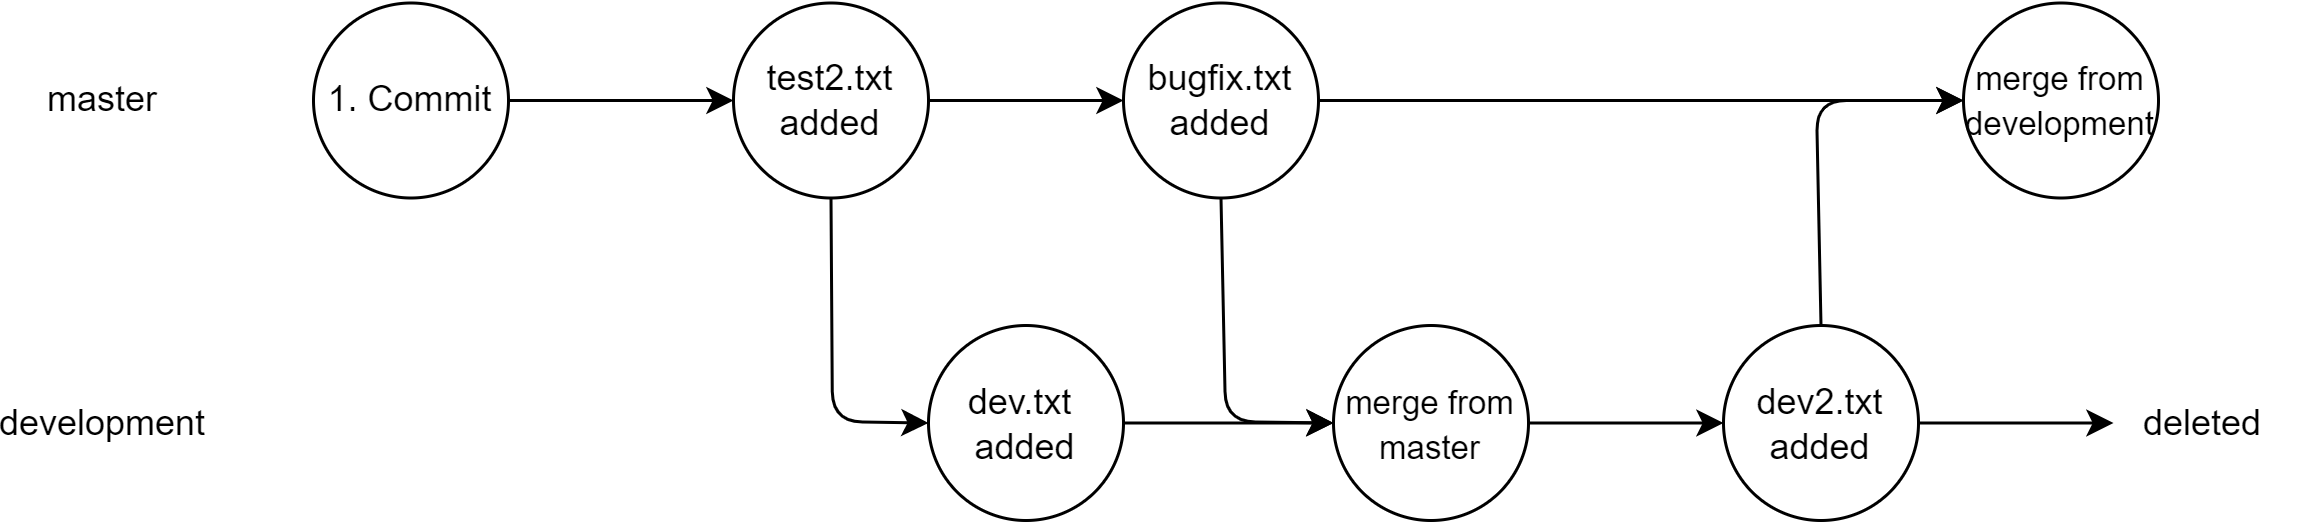
\includegraphics[scale=0.2]{../../media/git_example.png}
\end{center}

\textbf{Die gute Nachricht:} Alles was zuvor besprochen wurde muss nicht zwingend händisch ausgeführt werden (man versteht so aber besser was eigentlich passiert!) - VsCode nimmt uns viel der Arbeit ab und bietet eine graphische Oberfläche mit der wir ein Repository verwalten können, Details dazu im Unterricht bzw. im oben schon erwähnten Video,

\subsubsection{Github}
Bisher ist die Versionsverwaltung zwar nützlich für uns, aber noch nicht wirklich für die Verwendung in der Gruppe geeignet, da alles nur lokal auf den eigenen Rechnern passiert. Dieses \textbf{\href{https://youtu.be/YenryzR6xug}{Video}} zeigt die Grundlagen von Github und wie damit kollaborativ gearbeitet werden kann. 
\begin{center}
    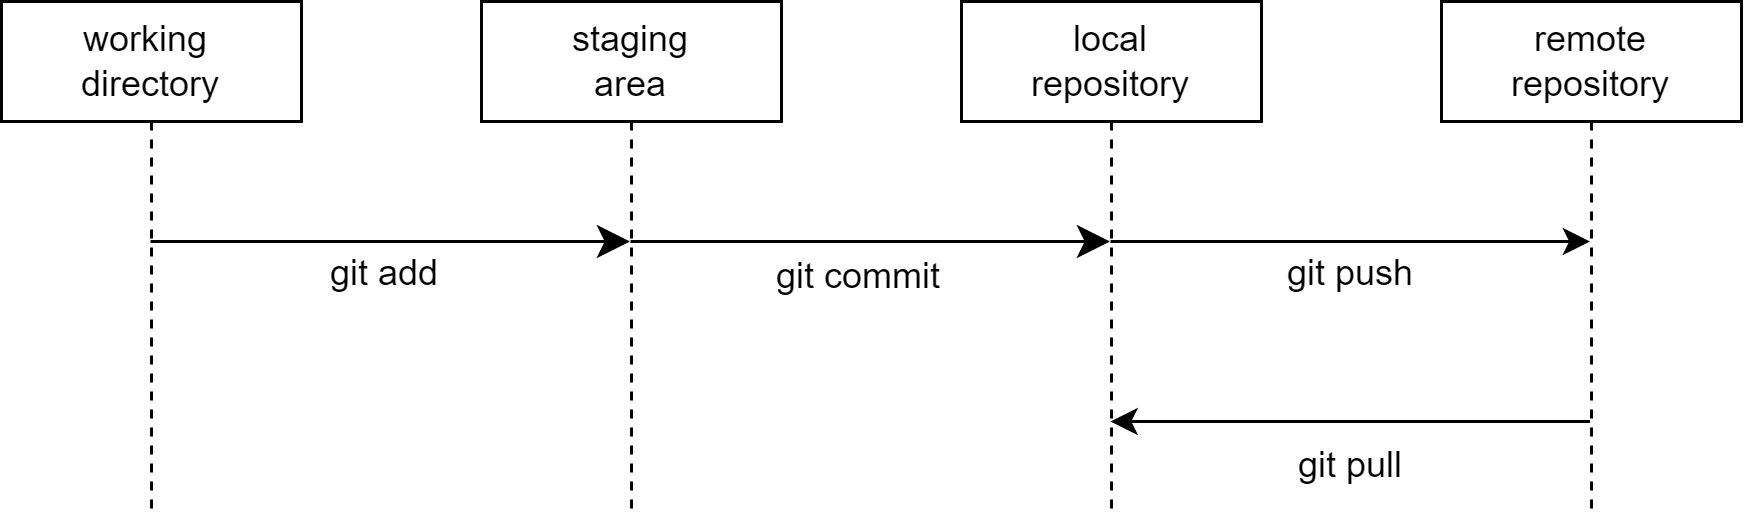
\includegraphics[scale=0.2]{../../media/push_pull.png}
\end{center}
Im Wesentlichen wird eine weitere Ebene hinzugefügt, das remote repository, das mit dem lokalen Repository via push und pull synchronisiert wird.
\subsection{User Stories und Aufgaben}
\label{sec:hwUserStories}

Nehmen wir an, das Projekt, das umgesetzt werden soll ist eine Form von Spiel, in diesem Fall Schach. Eine Beschreibung eines späteren Anwenders könnte dazu z.B. so ausfallen (im schlimmsten Fall wäre natürlich die Antwort: \q{Ich möchte Schach spielen können}, wir gehen aber von etwas detaillierteren Anforderungen aus):
\begin{enumerate}
    \item Man soll in einem Menü eine Schwierigkeit auswählen können und dann das Spiel starten.
    \item Die Schachfiguren sollen über das Brett bewegt werden können.
    \item Ich möchte sehen können, welche Züge ich mit welcher Figur machen kann. 
    \item Ein ungültiger Zug soll eindeutig erkennbar sein, wenn ich ihn versuche auszuführen. 
    \item Nach dem Spiel sollen die Züge des Gegners sichtbar sein, damit seine Strategie nachvollziehbar wird. 
    \item Eine Hilfefunktion wäre gut, die mir Grundlagen erklärt oder an bestimmten Stellen unter die Arme greift, wenn ich Hilfe brauche. 
    \item Ich möchte Spiele speichern und laden können.
\end{enumerate}

Diese User-Stories, also das umgangssprachliche definieren der Anforderungen sollte zunächst einmal festgehalten werden, handschriftlich oder - wenn gewünscht in einem Tool wie \textbf{\href{https://trello.com/}{Trello}} oder \textbf{\href{https://www.notion.so/de-de}{Notion}}. \\
Aus den User-Stories müssen jetzt konkrete Aufgaben für Entwicklys ausgearbeitet und priosiert werden. Nehmen wir an, es sind drei Teammitglieder beteiligt:
\begin{itemize}
    \item Monika: zuständig für das Model
    \item Viktor: zuständig für den View
    \item Claudia: zuständig für den Controller 
\end{itemize}

Analysieren wir zunächst die erste User Story:
\begin{center}
    Man soll in einem Menü eine Schwierigkeit auswählen können und dann das Spiel starten.
\end{center}
Ohne weitere Priorisierung könnte man daraus z.B.: folgende Aufgaben ableiten:
\begin{itemize}
    \item Viktor: \begin{itemize}
        \item erzeuge ein Spielfenster
        \item erzeuge ein Menü mit Spielstart und Schwierigkeitswahl
        \item erzeuge das Spielfeld
        \item erzeuge die Figuren
    \end{itemize}
    \item Monika: \begin{itemize}
        \item speichere Daten der Figuren
        \item speichere Daten des Spielfeldes bei Start 
        \item speichere Daten über den Schwierigkeitsgrad
    \end{itemize}
    \item Claudia: \begin{itemize}
        \item reagiere auf Schwierigkeitswahl 
        \item reagiere auf Spielstart
    \end{itemize}
\end{itemize}
Man kann unschwer erkennen, dass die meisten dieser Aufgaben weitere Fragen nach sich ziehen, die zunächst im Team besprochen werden müssen, z.B.:
\begin{itemize}
    \item Wie sollen die Daten gespeichert werden?
    \item Welche Schwierigkeitsstufen soll es geben?
    \item Wie sollen sich diese unterscheiden?
    \item In welcher Auflösung soll das Spielfeld und das Menü dargestellt werden?
    \item $\dots$
\end{itemize}

Es lassen sich dutzende weitere solcher Fragen stellen, deswegen ist eine \textbf{Priorisierung} unerlässlich. In obigem Beispiel: Die Auswahl und Verwendung unterschiedlicher Schwierigkeitsgrade ist zwar erstrebenswert, gehört aber zunächst nicht zur Grundfunktionalität eines Schachspiels, d.h. die Priorität sollte hier sicherlich für Viktor darauf liegen, Figuren und das Schachbrett vernünftig erzeugen und darstellen zu können. Monika muss sich darüber klar werden, wie die Figuren in den Daten repräsentiert werden. Claudia kann ohne die beiden Implementierungen noch nicht produktiv arbeiten, da der Controller auf bestehende Strukturen zugreifen muss, sie kann also entweder die anderen beiden unterstützen oder bereits ein Grundgerüst bauen, in das nur noch konkrete Methodennamen der beiden anderen Bereiche eingebaut werden müssen. \\
Eine übersichtlichere Möglichkeit, die Gedanken zu ordnen und kollaborativ daran zu arbeiten sind Concept Boards wie Trello:
\begin{center}
    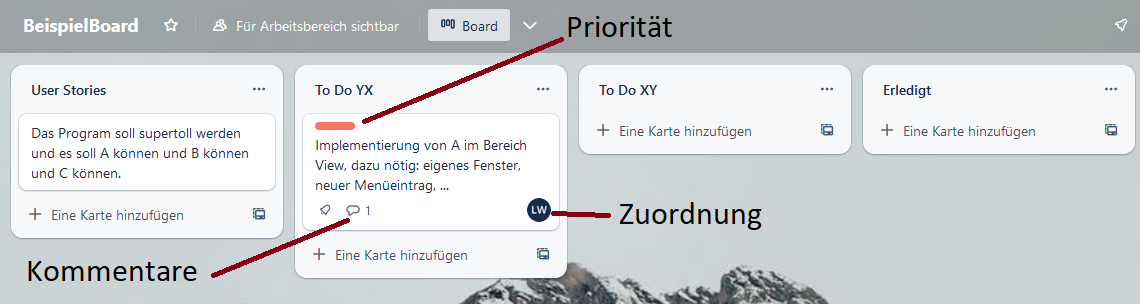
\includegraphics[scale=0.5]{../../media/trello.png}
\end{center}
Hier können die User Stories zuerst gesammelt werden und dann konkrete Aufgaben für Person YX oder XY daraus abgeleitet werden. Jeder Eintrag kann (hilfreich :) kommentiert werden oder es können weitere Zuordnungen der Aufgaben erfolgen, wenn sich ergibt, dass ein Bereich zur Lösung nicht ausreicht. Es können auch Priorisierungen vorgenommen werden (hier z.B. über ein Farbsystem geregelt). \\
Alternativ können auch Aufgabenlisten nach anderen Kriterien erstellt werden und es wird rein über die Zuordnung gearbeitet, je nachdem, wie die Arbeit für euch am effizientesten ablauft. \\
\textbf{Wichtig}: in irgendeiner Form \textbf{müssen} die Aufgaben verteilt und dokumentiert werden!

\subsection{Hinweise Model}
\label{sec:hwModel}

Wenn es an die Daten des Modells geht gibt es im Wesentlichen die drei bereits erwähnten Methoden, die auch im Schwierigkeitsgrad ansteigen. Grundsätzlich gibt es natürlich auch noch weitere Arten der Datenverwaltung, um den Rahmen jedoch nicht zu sprengen beschränken wir uns auf die \textbf{Datenklassen}, \textbf{JSON} und \textbf{SQL-Datenbanken}.
\vspace{-3mm}
\subsubsection{Datenklassen}

Jedwede Modellierung einer \q{natürlichen} Entität führte bereits bisher zu einer Art Datenklasse - z.B. die Klasse \q{Human}, die die Menschen in unserer Warteschlange repräsentiert haben. \\
Datenklassen zeichnen sich dadurch aus, dass sie keine weitere Logik enthalten außer die für diese Daten relevante, d.h. wir hatten beispspielsweise den Menschen:
\begin{minted}{java}
public class Human {
    String name;
    int age;

    public Human(String name, int age) {
        this.name=name;
        this.age =age;
    }

    //getter, setter, equals...

}
\end{minted}
Die einzige Aufgabe dieser Klasse ist es, die Daten, die einen Menschen charakterisieren zu verwalten. \\ 
Mit Java 14 gibt es ein neues Konstrukt, dass die Erstellung von Datenklassen etwas einfacher macht, die sogenannten \textbf{records}. Aus der offiziellen \href{https://docs.oracle.com/en/java/javase/14/language/records.html}{Hilfe} bzw. \href{https://docs.oracle.com/en/java/javase/17/docs/api/java.base/java/lang/Record.html}{Dokumentation} entnommen:
\begin{minted}{java}
record Rectangle(float length, float width){ }
\end{minted}
ist gleichbedeutend mit:
\begin{minted}{java}
final class Rectangle implements Shape {
    final double length;
    final double width;
    public Rectangle(double length, double width) {
        this.length = length;
        this.width = width;
    }
    double length() { return length; }
    double width() { return width; }
}
\end{minted}
Die Verwendung dieses Konstrukts ist natürlich nicht immer sinnvoll und auch nicht notwendig, die Erwähnung hier soll nur als Hinweis verstanden werden. \\
Möchte man nicht nur Daten verwalten, wie ein Objekt, also z.B. der Mensch aussieht, sondern auch konkrete Menschen in Klassen verwalten, könnte man das auch mit weiteren Klassen regeln (dies ist aber eher unüblich). \\
\textbf{Beispiel}: es soll ein ganzer Chor modelliert werden, neben Name und Alter wird in der Mensch-Klasse noch die Tonlage hinterlegt, das könnte z.B. so aussehen: 

\begin{minted}{java}
public class Choir {
    /*final damit der Choir nicht anderswo verändert werden kann, nur hier
    static, damit kein Objekt der Klasse Choir erzeugt werden muss, um auf 
    den Chor zuzugreifen */
    final static Human[] choir = {
        new Human("Horst", 55, "Bass");
        new Human("Angela", 60, "Alt");
        //...
    };
}
\end{minted}

\subsubsection{JSON}

JSON (JavaScript Object Notation) ist ein textbasiertes Datenformat. Die Daten werden hier in einem bestimmten Format in einer eigenen Datein (.json) abgespeichert. Die Syntax ist dabei relativ einfach zu lesen und zu verstehen, ein JSON-Datenobjekt wird immer durch geschweifte Klammern gekennzeichnet, ein Beispiel: 
\begin{minted}{json}
{
    "name": "Max Mustermann",
    "age": 30,
    "email": "max.mustermann@example.com",
    "address": {
        "street": "Musterstraße 123",
        "city": "Musterstadt",
        "country": "Deutschland"
    },
    "phoneNumbers": [
        "+49 123 456789",
        "+49 987 654321"
    ]
}     
\end{minted}
In JSON werden Daten in Form von Schlüssel-Wert-Paaren dargestellt, der Schlüssel steht dabei in Anführungszeichen, gefolgt von einem Doppelpunkt und den entsprechenden Werten (wenn es sich um Text handelt auch in Anführungszeichen!), einzelne Datenpunkte werden durch Kommata voneinander abgetrennt.  \\
In obigem Beispiel sieht man auch noch zwei weitere mögliche Notationen:
\begin{enumerate}
    \item \textbf{Die Adresse}: hinter dem Doppelpunkt der Adresse findet sich eine weitere geschweifte Klammer, das heißt die hinterlegten Daten können wieder ein \textbf{JSON-Objekt} sein. (man kann sie also beliebig tief \q{verschachteln}).
    \item \textbf{Die Telefonnummern}: hier befindet sich hinter dem Doppelpunkt eine eckige Klammer, das bedeutet, dass sich hier eine Liste an Werten findet. Der Unterschied wird insbesondere im Zugriff auf die Daten sichtbar, es gibt aber insbesondere keinen weiteren Schlüssel, der die Werte in der Liste charakterisiert, in der Adresse oben dagegen wird die Straße noch einmal explizit als \textbf{Schlüssel} hinterlegt.  
\end{enumerate}

Möchte man in Java mit JSON-Objekten umgeen, gibt es zum Beispiel die externe Bibliothek \textbf{org.json}, ein Anwendungsbeispiel: 

\begin{minted}{java}
import org.json.*;

public class Beispiel {
   public static void main(String[] args) {
      //JSON wird in einem Text definiert
      String jsonText = "{ \"name\": \"Max Mustermann\", \"age\": 30, 
      \"email\": \"max.mustermann@example.com\",
      \"address\": { \"street\": \"Musterstraße 123\",
      \"city\": \"Musterstadt\", \"country\": \"Deutschland\" },
      \"phoneNumbers\": [ \"+49 123 456789\", \"+49 987 654321\" ] }";
      
      //Es wird ein JSON-Objekt aus dem definierten Text gebaut. 
      JSONObject jsonObj = new JSONObject(jsonText);
      
      //Die Daten werden mit den passenden gettern ausgelesen...
      String name = jsonObj.getString("name");
      int age = jsonObj.getInt("age");
      String email = jsonObj.getString("email");
      String street = jsonObj.getJSONObject("address").getString("street");
      String city = jsonObj.getJSONObject("address").getString("city");
      String country = jsonObj.getJSONObject("address").getString("country");
      JSONArray phoneNumbers = jsonObj.getJSONArray("phoneNumbers");
      
      //... und ausgegeben
      System.out.println("Name: " + name);
      System.out.println("Alter: " + age);
      System.out.println("E-Mail: " + email);
      System.out.println("Straße: " + street);
      System.out.println("Stadt: " + city);
      System.out.println("Land: " + country);
      for (int i = 0; i < phoneNumbers.length(); i++) {
         String phoneNumber = phoneNumbers.getString(i);
         System.out.println("Telefonnummer " + (i+1) + ": " + phoneNumber);
      }
   }
}
\end{minted}
\newpage

In obigem Beispiel ist der JSON-Text noch im Code direkt angelegt, es ist aber natürlich noch möglich diesen in eine eigene Datei, z.B. data.json auszulagern: 
\begin{minted}{java}
    try {
         // Dateiinhalt in einen String lesen
         String jsonText = new String(Files.readAllBytes(Paths.get("data.json")));
         
         // ... wie oben
      } catch (Exception e) {
         System.err.println("Fehler beim Lesen der JSON-Datei: " + e.getMessage());
      }
\end{minted}
\textbf{Achtung:} der Pfad ist relativ zum root-Verzeichnis des Projekts zu verstehen, liegen die Daten also in einem Unterordner, so muss dieser in den PFad eingebettet werden, z.B.: \q{ordner/data.json}. \\
Allgemein lässt sich sagen, dass die Verwendung von JSON mit Java häufig etwas umständlich wirkt, aber dennoch vernünftig funktioniert.  \\

\subsubsection{SQL-Datenbanken - nur für Experten}

Es ist unwahrscheinlich, dass bei einem der Projekte die Verwendung einer Datenbank notwendig wird, aber der Vollständigkeit halber sei diese Möglichkeit erwähnt. Man kann aus Java direkt auf eine existierende SQL-Datenbank zugreifen, der Prozess ist aber häufig trickreich und fehleranfällig. Eine vernünftige Übersicht findet sich z.B. \href{https://www.baeldung.com/java-connect-mysql}{hier}. Ich empfehle die Verwendung von JDBC, also der ersten Option, wenn gewünscht. \\
Anbei ein Anschauungsbeispiel, wie mit JDBC ein Login-System realisiert wurde: 
\begin{minted}{java}
import java.math.BigInteger;
import java.nio.charset.StandardCharsets;
import java.security.MessageDigest;
import java.security.NoSuchAlgorithmException;
import java.sql.Connection;
import java.sql.DriverManager;
import java.sql.PreparedStatement;
import java.sql.ResultSet;
import java.sql.SQLException;

public class DatabaseConnect {
    
    private static final String DB_PASSWORD = "password";
    private static final String DB_USERNAME = "client";


    public static void setPassword(String username, String password) {
        String sqlSetPassword = "INSERT INTO login VALUES (?, ?)";
        String hashedPassword = buildPasswordString(password);
        Connection con = connect();
        try {
            PreparedStatement ps = con.prepareStatement(sqlSetPassword);
            ps.setString(1, username);
            ps.setString(2, hashedPassword);
            ps.executeUpdate();
            con.close();
        } catch (SQLException e) {
            e.printStackTrace();
        }
    }

    public static void updatePassword(String username, String password) {
        String sqlUpdatePassword = "UPDATE login SET `Password` = ?  WHERE `Username` = ?";
        String hashedPassword = buildPasswordString(password);
        Connection con = connect();
        try{
            PreparedStatement ps = con.prepareStatement(sqlUpdatePassword);
            ps.setString(1, hashedPassword);
            ps.setString(2, username);
            ps.executeUpdate();
            con.close();
        } catch(SQLException e) {
            e.printStackTrace();
        }
    }

    public static boolean login(String username, String password) {
        String sqlFetchPassword = "SELECT `password` FROM login WHERE `Username` = ?";
        String hashedLoginPassword = buildPasswordString(password);
        Connection con = connect();
        try {
            PreparedStatement ps = con.prepareStatement(sqlFetchPassword);
            ps.setString(1, username);
            ResultSet results = ps.executeQuery();
            results.next();
            String databasePassword = results.getString(1);
            con.close();
            if(databasePassword.equals(hashedLoginPassword)) return true; 
        } catch (SQLException e) {
            e.printStackTrace();
        }
        return false;
    } 

    private static String buildPasswordString(String password) {
        BigInteger bigInteger = null;
        try {
            bigInteger = new BigInteger(1, getSHA(password));
        } catch (NoSuchAlgorithmException e) {
            e.printStackTrace();
        }
        StringBuilder hexString = new StringBuilder(bigInteger.toString(16));
        while(hexString.length() < 64) {
            hexString.insert(0, '0');
        }
        return hexString.toString();
    }

    private static byte[] getSHA(String input) throws NoSuchAlgorithmException {
        MessageDigest md = MessageDigest.getInstance("SHA-256");
        return md.digest(input.getBytes(StandardCharsets.UTF_8));
    }
    
    private static Connection connect(){
        String CONNECTION_URL = "jdbc:mysql://localhost:3306/database";
        Connection con = null;
        try{
            con = DriverManager.getConnection(CONNECTION_URL, DB_USERNAME, DB_PASSWORD);
        } catch(SQLException e) {
            e.printStackTrace();
        }
        return con;
    }

}
\end{minted}


\subsection{Hinweise View}
\label{sec:hwView}
Ähnlich wie beim Model gibt es verschiedene Wege, die man einschlagen kann, um dem User eine Interaktion mit dem Program zu ermöglichen. Wie oben steigt dabei der Schwierigkeitsgrad der vorgestellten methoden tendenziell an. 

\subsubsection{Konsole}

Beginnen wir mit der einfachsten Methode, der Asugabe und Interaktion über die Konsole. Diese Möglichkeit haben wir durch die Verwendung von System.out.println() schon sehr häufig verwendet. Grundsätzlich spricht natürlich nichts dagegen den Anwender so mit dem Program kommunizieren lassen, jedoch haben sich - gerade im Windows-Bereich - die graphischen Oberflächen für die Mehrheit der Bevölkerung durchgesetzt. Wollt ihr trotzdem diesen Weg gehen, dann sei an die Scanner-Klasse erinnert, damit auf Eingaben des Benutzers reagiert werden kann, z.B.:
\begin{minted}{java}
import java.util.Scanner;

public class ScannerExample {
    public static void main(String[] args) {
        // Erstelle einen neuen Scanner, der auf System.in (Standard-Eingabe) liest
        Scanner scanner = new Scanner(System.in);

        // Lese die nächste Zeile der Eingabe
        System.out.println("Bitte geben Sie Ihren Namen ein:");
        String name = scanner.nextLine();

        // Lese eine eingegebene 
        System.out.println("Bitte geben Sie Ihr Alter ein:");
        int age = scanner.nextInt();

        // Gib den Namen und das Alter aus
        System.out.println("Sie sind " + name + " und sind" + age + " Jahre alt.");

        // Schließe den Scanner
        scanner.close();
    }
}

\end{minted}


\subsubsection{Swing}
Eine der klassischen Methoden Graphical User Interfaces (GUIs) in Java zu schreiben ist die Swing-Bibliothek. Sie kommt bereits mit der Standard-Bibliothek und kann direkt verwendet werden, die grundlegende Syntax ist nicht schwer, der folgende Code erzeugt ein Fenster mit einem Label:
\newpage

\begin{minted}{java}
import javax.swing.*;

public class SwingDemo {

    public static void main(String[] args) {
        JFrame frame = new JFrame("Meine SWING-Applikation");
        frame.setSize(400, 300);
        frame.setDefaultCloseOperation(JFrame.EXIT_ON_CLOSE);

        JLabel label = new JLabel("Hello World!");
        frame.add(label);
        frame.setVisible(true);
    }
}
\end{minted}

Im Wesentlichen ist das Hauptfenster ein Frame, der als Breite den absoluten Wert 400px und als Höhe den Wert 300px bekommt. Wenn wir auf das bekannte X klicken wird beendet und zu unserem Frame wird ein Label hinzugefügt. Am Ende der Methode wird der Frame sichtbar \q{geschalten}. \\
Leider bleibt es nicht ganz so einfach, insbesondere die Interaktion mit dem Benutzer ist in den Implementierungen in Java zuerst etwas unübersichtlich, fügen wir einen Button nach unserem Label hinzu, der das Label ein- bzw. ausblenden soll. 
\begin{minted}{java}
JButton button = new JButton("Hide/Show Label");
button.addActionListener(new ActionListener() {
    @Override
    public void actionPerformed(ActionEvent e) {
        if (label.isVisible()) {
            label.setVisible(false);
        } else {
            label.setVisible(true);
        }
    }
});
frame.add(button, BorderLayout.SOUTH);
\end{minted}
Betrachten wir zuerst die letzte Zeile, der Button wird wieder dem Frame hinzugefügt, jetzt aber im \q{Süden}, also am unteren Ende unseres Rahmens. Allgemein werden die Positionen in sogenannten Layouts verwaltet, die als Container für die einzelnen graphischen Objekte dienen. Je nachdem wie man die Anordnung haben möchte gibt es verschiedene Klassen, z.B. das obige BorderLayout, dass die Komponenten in fünf Bereichen anordnet: Norden, Süden, Osten, Westen und Mitte. \\
Jetzt zum komplizierteren Teil, zunächst erzeugen wir einen neuen Button mit seinem Text. Würde man den Rest des Codes weglassen wäre dieser Button aber funktionslos, der Konstruktor erzeugt nur das graphische Element, das auch angezeigt wird, stattet es aber noch \textbf{nicht} mit Funktion aus. \\
Das passiert erst in der nächsten Zeile, wir wollen einen sogenannten \textbf{ActionListener} hinzufügen, d.h. wenn etwas mit dem Button passiert, möchten wir eine Aktion auslösen. \vspace{2mm}\\
\textbf{Hinweis:} Wollen wir beispielsweise nur auf Maus-Eingaben reagieren, so könnte alternativ ein MouseListener hinzugefügt werden. \vspace{2mm}\\
Wir möchten natürlich nicht, dass einfach irgendetwas passiert, sondern unseren eigenen ActionListener definieren. Hier wird es etwas trickreicher: ActionListener ist eigentlich ein Interface, das fordert, dass eine Methode \textit{actionPerformed()} implementiert wird. Wir möchten aber nicht für jeden unserer Listener eine eigene Klasse irgendwo in unserem Code haben, sondern möglichst an genau dieser Stelle den Listener implementieren. Dazu wird eine sogenannte \textbf{anonyme innere Klasse} verwendet. Wir sehen oben, dass nach Aufruf des Konstruktors eine geschweifte Klammer aufgeht, wir definieren also eine weitere - nicht benannte (deswegen auch \q{anonym}) - Klasse direkt in unserem Code (deswegen \q{innere}), diese anonyme innere Klasse implementiert das ActionListener-Interface und wir überschreiben die \textbf{actionPerformed()} - Methode so wie wir sie wollen: \\

ist das Label sichtbar, wird es versteckt, andernfalls wieder sichtbar gemacht. \\

\textbf{Hinweis:} Wir kümmern uns nicht darum, was genau das zugehörige ActionEvent war, deswegen greifen wir innerhalb der \textit{actionPerformed()}-Methode auch nicht auf den Eingabeparameter $e$ zu, der das Event, also das Ereignis repräsentiert! \\

Dieses Beispiel stellt natürlich nur einen sehr, sehr kleinen Einblick in die Welt von Swing dar, sollte aber als Ausgangspunkt genügen, um von hier aus weiter zu arbeiten. Es gibt unzählige Tutorials im Internet, eine Auswahl (nicht streng auf Tauglichkeit geprüft):
\begin{enumerate}
    \item \href{https://www.javatpoint.com/java-swing}{\textbf{Javatpoint}}: textbasiertes Tutorial, geht nacheinander auf verschiedene Objekte ein, gut als Nachschlagewerk mit Beispielen geeignet. 
    \item \href{https://www.geeksforgeeks.org/introduction-to-java-swing/}{\textbf{geeksforgeeks}}: textbasiert, weniger übersichtlich strukturiert, aber viele Artikel.
    \item  \href{https://docs.oracle.com/javase/7/docs/api/javax/swing/package-summary.html}{\textbf{Offizielle Doumentation}}: wenn Details genau nachgelesen werden müssen. 
    \item \href{https://www.youtube.com/playlist?list=PLNmsVeXQZj7o5ALam15-pQWtf22RgU6D7}{\textbf{Morpheus}}: Youtube-Reihe. Sehr ausführlich, aber schon etwas älter. 
    \item \href{https://www.youtube.com/playlist?list=PL3bGLnkkGnuV699lP_f9DvxyK5lMFpq6U}{\textbf{Java Code Junkie}}: Youtube-Reihe, ebenfalls ausführlich, etwas aktueller.
    \item Allgemein: Google/ChatGPT/Youtube: ihr wisst wie das geht :)
\end{enumerate}

\subsubsection{JavaFX - für Experten}

Etwas moderner, aber noch etwas umfangreicher in der Gestaltung als Swing ist JavaFX. Entscheidet man sich für diesen Ansatz, so sollte direkt das Ganze Projekt als JavaFX Projekt angelegt werden, da sich Abhängigkeiten ergeben, die nicht von der Standardbibliothek abgedeckt werden. Wird mit VSCode gearbeitet finden sich als Einstiegspunkt \href{https://code.visualstudio.com/docs/java/java-gui}{hier} Hinweise, sodass die entsprechenden Abhängigkeiten automatisch eingebaut sind. \\
Auch für JavaFX gibt es zahlreiche Tutorials (ebenfalls nicht vollständig geprüft):
\begin{enumerate}
    \item \href{https://docs.oracle.com/javafx/2/get_started/jfxpub-get_started.htm}{\textbf{Offizielles Oracle Tutorial}}: referenziert die NetBeans IDE, natürlich auch mit anderen IDEs möglich. 
    \item \href{https://www.javatpoint.com/javafx-tutorial}{\textbf{Javatpoint}}: textbasiertes Tutorial, geht nacheinander auf verschiedene Objekte ein, gut als Nachschlagewerk mit Beispielen geeignet.
    \item \href{https://www.geeksforgeeks.org/javafx-tutorial/}{\textbf{geeksforgeeks}}: textbasiert, weniger übersichtlich strukturiert, aber viele Artikel. 
    \item  \href{https://docs.oracle.com/javafx/2/}{\textbf{Offizielle Doumentation}}: wenn Details genau nachgelesen werden müssen. 
    \item \href{https://www.youtube.com/playlist?list=PL7Rswbug-Foa9BwgUNxUUoVr15bbCIqTj}{\textbf{ITCademy}}: Youtube-Reihe, relativ ausführlich und aktuell.
    \item Allgemein: Google/ChatGPT/Youtube: ihr wisst wie das geht :)
\end{enumerate}

\subsection{Hinweise Controller}
\label{sec:hwController}

Im Gegensatz zu Model und View lassen sich für den Controller keine generellen Empfehlungen für den Anfang geben, da es stark auf die Implementierungen der anderen beiden Bereiche ankommt, wie Methoden geschrieben werden. \\
Es empfiehlt sich, dass in der Anfangsphase des Projekts das Teammitglied, das als Hauptbereich den Controller hat die anderen Teammitglieder unterstützt, je nachdem wo die größeren Probleme vorliegen. 
\newpage
\subsection{Ideensammlung für Projekte}
\label{sec:ideen}

\textbf{Hinweis:} Idealerweise sollte das Projekt natürlich im zeitlichen Rahmen beendet werden, sollte das aufgrund des Umfangs nicht möglich sein muss das nicht zwangsläufig zu Punktabzug führen. Es muss aber eine Grundfunktionalität hergestellt werden, damit erkennbar ist, dass das Projekt grundsätzlich erfolgreich verläuft und nur noch nicht \q{vollständig} ist. 

\begin{enumerate}
    \item \textbf{Spiele} in verschiedenster Form: text based adventure, Quizspiel, Kartenspiel, etc. Der Phantasie sind keine Grenzen gesetzt,...
    \item \textbf{Verwaltungssoftware}: für Noten, Rezepte, Inventar, Bibliothek,...
    \item \textbf{Physikalische Simulationen}: Simulation verschiedern physikalischer Gesetze, grafische Veranschaulichung,...
    \item \textbf{Ploten}: Das ganz eigene Geogebra, oder ein kleiner Mathehelfer,...
    \item \textbf{Lernprogram}: Ein interaktives Program zum Vokabeln lernen, oder vielleicht für Chemie-Formeln,...
\end{enumerate}

\end{document}